\documentclass{standalone}
\usepackage{tikz}
\usetikzlibrary{patterns, positioning}


\begin{document}
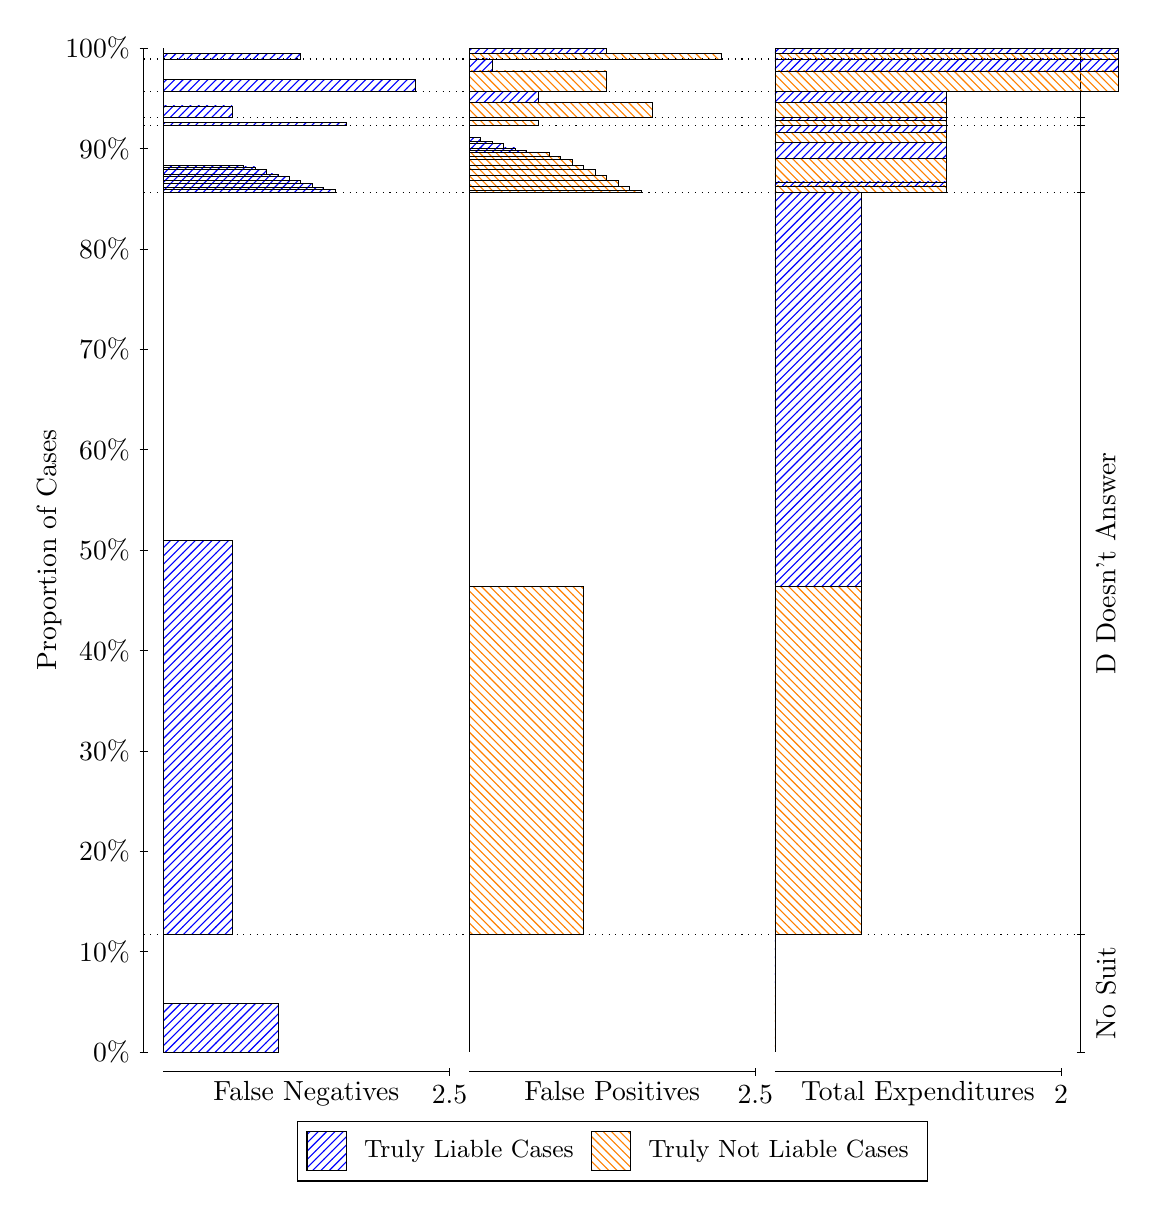
\begin{tikzpicture}
\draw[black, very thin] (1.5,1.75) -- (1.5,14.5);
\node[rotate=90, text=black, anchor=center] at (0.3, 8.125) {Proportion of Cases};
\draw[black, very thin] (1.45,1.75) -- (1.55,1.75);
\node[text=black, anchor=east] at (1.45, 1.75) {0\%};
\draw[black, very thin] (1.45,3.025) -- (1.55,3.025);
\node[text=black, anchor=east] at (1.45, 3.025) {10\%};
\draw[black, very thin] (1.45,4.3) -- (1.55,4.3);
\node[text=black, anchor=east] at (1.45, 4.3) {20\%};
\draw[black, very thin] (1.45,5.575) -- (1.55,5.575);
\node[text=black, anchor=east] at (1.45, 5.575) {30\%};
\draw[black, very thin] (1.45,6.85) -- (1.55,6.85);
\node[text=black, anchor=east] at (1.45, 6.85) {40\%};
\draw[black, very thin] (1.45,8.125) -- (1.55,8.125);
\node[text=black, anchor=east] at (1.45, 8.125) {50\%};
\draw[black, very thin] (1.45,9.4) -- (1.55,9.4);
\node[text=black, anchor=east] at (1.45, 9.4) {60\%};
\draw[black, very thin] (1.45,10.675) -- (1.55,10.675);
\node[text=black, anchor=east] at (1.45, 10.675) {70\%};
\draw[black, very thin] (1.45,11.95) -- (1.55,11.95);
\node[text=black, anchor=east] at (1.45, 11.95) {80\%};
\draw[black, very thin] (1.45,13.225) -- (1.55,13.225);
\node[text=black, anchor=east] at (1.45, 13.225) {90\%};
\draw[black, very thin] (1.45,14.5) -- (1.55,14.5);
\node[text=black, anchor=east] at (1.45, 14.5) {100\%};

\draw[black, very thin] (13.4,1.75) -- (13.4,14.5);
\draw[black, very thin] (13.35,1.75) -- (13.45,1.75);
\node[anchor=west] at (13.35, 1.75) {};
\draw[black, very thin] (13.35,3.2422) -- (13.45,3.2422);
\node[anchor=west] at (13.35, 3.2422) {};
\draw[black, very thin] (13.35,12.669) -- (13.45,12.669);
\node[anchor=west] at (13.35, 12.669) {};
\draw[black, very thin] (13.35,13.517) -- (13.45,13.517);
\node[anchor=west] at (13.35, 13.517) {};
\draw[black, very thin] (13.35,13.62) -- (13.45,13.62);
\node[anchor=west] at (13.35, 13.62) {};
\draw[black, very thin] (13.35,13.948) -- (13.45,13.948);
\node[anchor=west] at (13.35, 13.948) {};
\draw[black, very thin] (13.35,14.361) -- (13.45,14.361);
\node[anchor=west] at (13.35, 14.361) {};
\draw[black, very thin] (13.35,14.5) -- (13.45,14.5);
\node[anchor=west] at (13.35, 14.5) {};

\draw[black, very thin, pattern color=blue, pattern=north east lines] (1.75,1.75) rectangle (3.2033,2.3683);
\draw[black, very thin, pattern color=orange, pattern=north west lines] (1.75,2.3683) rectangle (1.75,3.2422);
\draw[black, very thin, pattern color=blue, pattern=north east lines] (1.75,3.2422) rectangle (2.622,8.2493);
\draw[black, very thin, pattern color=orange, pattern=north west lines] (1.75,8.2493) rectangle (1.75,12.669);
\draw[black, very thin, pattern color=blue, pattern=north east lines] (1.75,12.669) rectangle (3.93,12.703);
\draw[black, very thin, pattern color=blue, pattern=north east lines] (1.75,12.703) rectangle (3.7847,12.73);
\draw[black, very thin, pattern color=blue, pattern=north east lines] (1.75,12.73) rectangle (3.6393,12.781);
\draw[black, very thin, pattern color=blue, pattern=north east lines] (1.75,12.781) rectangle (3.494,12.816);
\draw[black, very thin, pattern color=blue, pattern=north east lines] (1.75,12.816) rectangle (3.3487,12.867);
\draw[black, very thin, pattern color=blue, pattern=north east lines] (1.75,12.867) rectangle (3.2033,12.902);
\draw[black, very thin, pattern color=blue, pattern=north east lines] (1.75,12.902) rectangle (3.058,12.954);
\draw[black, very thin, pattern color=blue, pattern=north east lines] (1.75,12.954) rectangle (2.9127,12.99);
\draw[black, very thin, pattern color=blue, pattern=north east lines] (1.75,12.99) rectangle (2.7673,13.013);
\draw[black, very thin, pattern color=orange, pattern=north west lines] (1.75,13.013) rectangle (1.75,13.517);
\draw[black, very thin, pattern color=blue, pattern=north east lines] (1.75,13.517) rectangle (4.0753,13.555);
\draw[black, very thin, pattern color=orange, pattern=north west lines] (1.75,13.555) rectangle (1.75,13.62);
\draw[black, very thin, pattern color=blue, pattern=north east lines] (1.75,13.62) rectangle (2.622,13.764);
\draw[black, very thin, pattern color=orange, pattern=north west lines] (1.75,13.764) rectangle (1.75,13.948);
\draw[black, very thin, pattern color=blue, pattern=north east lines] (1.75,13.948) rectangle (4.9473,14.101);
\draw[black, very thin, pattern color=orange, pattern=north west lines] (1.75,14.101) rectangle (1.75,14.361);
\draw[black, very thin, pattern color=blue, pattern=north east lines] (1.75,14.361) rectangle (3.494,14.433);
\draw[black, very thin, pattern color=orange, pattern=north west lines] (1.75,14.433) rectangle (1.75,14.5);
\draw[black, very thin, pattern color=orange, pattern=north west lines] (5.6333,1.75) rectangle (5.6333,2.6239);
\draw[black, very thin, pattern color=blue, pattern=north east lines] (5.6333,2.6239) rectangle (5.6333,3.2422);
\draw[black, very thin, pattern color=orange, pattern=north west lines] (5.6333,3.2422) rectangle (7.0867,7.6624);
\draw[black, very thin, pattern color=blue, pattern=north east lines] (5.6333,7.6624) rectangle (5.6333,12.669);
\draw[black, very thin, pattern color=orange, pattern=north west lines] (5.6333,12.669) rectangle (7.8133,12.696);
\draw[black, very thin, pattern color=orange, pattern=north west lines] (5.6333,12.696) rectangle (7.668,12.745);
\draw[black, very thin, pattern color=orange, pattern=north west lines] (5.6333,12.745) rectangle (7.5227,12.82);
\draw[black, very thin, pattern color=orange, pattern=north west lines] (5.6333,12.82) rectangle (7.3773,12.878);
\draw[black, very thin, pattern color=orange, pattern=north west lines] (5.6333,12.878) rectangle (7.232,12.956);
\draw[black, very thin, pattern color=orange, pattern=north west lines] (5.6333,12.956) rectangle (7.0867,13.009);
\draw[black, very thin, pattern color=orange, pattern=north west lines] (5.6333,13.009) rectangle (6.9413,13.089);
\draw[black, very thin, pattern color=orange, pattern=north west lines] (5.6333,13.089) rectangle (6.796,13.128);
\draw[black, very thin, pattern color=orange, pattern=north west lines] (5.6333,13.128) rectangle (6.6507,13.174);
\draw[black, very thin, pattern color=blue, pattern=north east lines] (5.6333,13.174) rectangle (6.36,13.196);
\draw[black, very thin, pattern color=blue, pattern=north east lines] (5.6333,13.196) rectangle (6.2147,13.232);
\draw[black, very thin, pattern color=blue, pattern=north east lines] (5.6333,13.232) rectangle (6.0693,13.285);
\draw[black, very thin, pattern color=blue, pattern=north east lines] (5.6333,13.285) rectangle (5.924,13.319);
\draw[black, very thin, pattern color=blue, pattern=north east lines] (5.6333,13.319) rectangle (5.7787,13.37);
\draw[black, very thin, pattern color=blue, pattern=north east lines] (5.6333,13.37) rectangle (5.6333,13.517);
\draw[black, very thin, pattern color=orange, pattern=north west lines] (5.6333,13.517) rectangle (6.5053,13.581);
\draw[black, very thin, pattern color=blue, pattern=north east lines] (5.6333,13.581) rectangle (5.6333,13.62);
\draw[black, very thin, pattern color=orange, pattern=north west lines] (5.6333,13.62) rectangle (7.9587,13.805);
\draw[black, very thin, pattern color=blue, pattern=north east lines] (5.6333,13.805) rectangle (6.5053,13.948);
\draw[black, very thin, pattern color=orange, pattern=north west lines] (5.6333,13.948) rectangle (7.3773,14.209);
\draw[black, very thin, pattern color=blue, pattern=north east lines] (5.6333,14.209) rectangle (5.924,14.361);
\draw[black, very thin, pattern color=orange, pattern=north west lines] (5.6333,14.361) rectangle (8.8307,14.428);
\draw[black, very thin, pattern color=blue, pattern=north east lines] (5.6333,14.428) rectangle (7.3773,14.5);
\draw[black, very thin, pattern color=orange, pattern=north west lines] (9.5167,1.75) rectangle (9.5167,2.6239);
\draw[black, very thin, pattern color=blue, pattern=north east lines] (9.5167,2.6239) rectangle (9.5167,3.2422);
\draw[black, very thin, pattern color=orange, pattern=north west lines] (9.5167,3.2422) rectangle (10.607,7.6624);
\draw[black, very thin, pattern color=blue, pattern=north east lines] (9.5167,7.6624) rectangle (10.607,12.669);
\draw[black, very thin, pattern color=orange, pattern=north west lines] (9.5167,12.669) rectangle (11.697,12.748);
\draw[black, very thin, pattern color=blue, pattern=north east lines] (9.5167,12.748) rectangle (11.697,12.799);
\draw[black, very thin, pattern color=orange, pattern=north west lines] (9.5167,12.799) rectangle (11.697,13.1);
\draw[black, very thin, pattern color=blue, pattern=north east lines] (9.5167,13.1) rectangle (11.697,13.304);
\draw[black, very thin, pattern color=orange, pattern=north west lines] (9.5167,13.304) rectangle (11.697,13.428);
\draw[black, very thin, pattern color=blue, pattern=north east lines] (9.5167,13.428) rectangle (11.697,13.517);
\draw[black, very thin, pattern color=orange, pattern=north west lines] (9.5167,13.517) rectangle (11.697,13.581);
\draw[black, very thin, pattern color=blue, pattern=north east lines] (9.5167,13.581) rectangle (11.697,13.62);
\draw[black, very thin, pattern color=orange, pattern=north west lines] (9.5167,13.62) rectangle (11.697,13.805);
\draw[black, very thin, pattern color=blue, pattern=north east lines] (9.5167,13.805) rectangle (11.697,13.948);
\draw[black, very thin, pattern color=orange, pattern=north west lines] (9.5167,13.948) rectangle (13.877,14.209);
\draw[black, very thin, pattern color=blue, pattern=north east lines] (9.5167,14.209) rectangle (13.877,14.361);
\draw[black, very thin, pattern color=orange, pattern=north west lines] (9.5167,14.361) rectangle (13.877,14.428);
\draw[black, very thin, pattern color=blue, pattern=north east lines] (9.5167,14.428) rectangle (13.877,14.5);
\draw[black, dotted] (1.5,3.2422) -- (13.4,3.2422);
\draw[black, dotted] (1.5,12.669) -- (13.4,12.669);
\draw[black, dotted] (1.5,13.517) -- (13.4,13.517);
\draw[black, dotted] (1.5,13.62) -- (13.4,13.62);
\draw[black, dotted] (1.5,13.948) -- (13.4,13.948);
\draw[black, dotted] (1.5,14.361) -- (13.4,14.361);
\draw[black, very thin] (1.75,1.5) -- (5.3833,1.5);
\node[text=black, anchor=north] at (3.5667, 1.5) {False Negatives};
\draw[black, very thin] (5.3833,1.45) -- (5.3833,1.55);
\node[text=black, anchor=north] at (5.3833, 1.45) {2.5};

\draw[black, very thin] (5.6333,1.5) -- (9.2667,1.5);
\node[text=black, anchor=north] at (7.45, 1.5) {False Positives};
\draw[black, very thin] (9.2667,1.45) -- (9.2667,1.55);
\node[text=black, anchor=north] at (9.2667, 1.45) {2.5};

\draw[black, very thin] (9.5167,1.5) -- (13.15,1.5);
\node[text=black, anchor=north] at (11.333, 1.5) {Total Expenditures};
\draw[black, very thin] (13.15,1.45) -- (13.15,1.55);
\node[text=black, anchor=north] at (13.15, 1.45) {2};

\node[text=black, centered, rotate=90] at (13.72, 2.4961) {No Suit};
\node[text=black, centered, rotate=90] at (13.72, 7.9558) {D Doesn't Answer};






\draw (7.449999999999999,1.5) node[draw=none] (baseCoordinate) {};
\begin{scope}[align=center]
        \matrix[scale=0.5, draw=black, below=0.5cm of baseCoordinate, nodes={draw}, column sep=0.1cm]{
            \node[rectangle, draw, minimum width=0.5cm, minimum height=0.5cm, pattern color=blue, pattern=north east lines] {}; &
            \node[draw=none, font=\small, text=black] (B) {Truly Liable Cases}; &
            \node[rectangle, draw, minimum width=0.5cm, minimum height=0.5cm, pattern color=orange, pattern=north west lines] {}; &
            \node[draw=none, font=\small, text=black] (B) {Truly Not Liable Cases}; \\
            };
\end{scope}

\end{tikzpicture}
\end{document}